\documentclass[Arkitektur/System_main.tex]{subfiles}

\begin{document}
\section{Hardwarearkitektur} \label{sec:hardware_arkitektur}

I dette afsnit beskrives hardwarearkitekturen for Beer Pong bordet. Systemets struktur er illustreret ved hjælp af blokdefinitions diagrammer (BDD). De viser hvordan systemet er sammensat, herunder hvilke dele det består af, og antallet af dele. Et overordnet BDD for systemet er vist i figur \ref{fig:overall_hardware_bdd}. Blokkene og deres funktion er nærmere specificeret i en blokbeskrivelse. Derudover er der lavet et overordnet internt blokdiagram (IBD), som viser bordets grænseflader, og hvordan blokkene er internt forbundet med hinanden. Særligt blokkene Player side og Ball dispenser er essentielle for spillets afvikling. Der er udarbejdet separate diagrammer for disse - Player side er vist i afsnit \ref{sec:playerside_hardware}, mens Ball dispenser kan ses i afsnit \ref{sec:balldispenser_hardware}.

\subsection{Overordnet} \label{sec:overall_hardware}
\subsubsection{Blok definitionsdiagram - \nameref{sec:overall_hardware}} \label{sec:overall_hardware_bdd}
\begin{figure}[H]
    \centering
    \makebox[\textwidth][c]{%
        \includegraphics[width=1.3\columnwidth,trim={0.24in 0.24in 0.24in 0.24in},clip, page=2]{Arkitektur/graphics/BDD_og_IBD.pdf}
    }
    \caption{Overordnet blok definitionsdiagram for systemet.}
    \label{fig:overall_hardware_bdd}
\end{figure}

\subsubsection{Blokbeskrivelse - \nameref{sec:overall_hardware}} \label{sec:overall_hardware_block_description}

\begin{table}[H]
\centering
\begin{tabular}{|L{0.2\columnwidth}|L{0.7\columnwidth}|}
\hline
\textbf{Blok} & \textbf{Beskrivelse} \\ \hline
Player side & Se afsnit \textit{\nameref{sec:systemarkitektur}} \\ \hline
RPi & Se afsnit \textit{\nameref{sec:systemarkitektur}}  \\ \hline
Display & Denne komponent er købt ind udefra, og udvikles ikke som en del af projektet. Display er placeret i midten af bordet og skal vise information til brugerne. Er forbundet til RPi, og det der vises er styret af den. \\ \hline
Ball dispenser & Se afsnit \textit{\nameref{sec:systemarkitektur}}   \\ \hline
\end{tabular}
\end{table}

\subsubsection{Intern blokdiagram - \nameref{sec:overall_hardware}} \label{sec:overall_hardware_ibd}

På figur \ref{fig:overall_hardware_ibd} ses et ibd for det overordnede system, hvor signaler er vist.

\begin{figure}[H]
    \centering
    \makebox[\textwidth][c]{%
        \includegraphics[width=1.3\columnwidth,trim={0.24in 0.24in 0.24in 0.24in},clip, page=5]{Arkitektur/graphics/BDD_og_IBD.pdf}
    }
    \caption{Overordnet intern blokdiagram for systemet.}
    \label{fig:overall_hardware_ibd}
\end{figure}

\subsubsection{Port beskrivelse - Beerpong table}
\begin{longtable}{|L{0.2\textwidth}|L{0.2\textwidth}|L{0.2\textwidth}|L{0.3\textwidth}|}
\hline
\textbf{blok navn}                            & \textbf{port navn}         & \textbf{port type} & \textbf{port beskrivelse}                                                                          \\ \hline
\multirow{2}{*}{Display}      & 230V                & AC        & forsyner display                                      \\ \cline{2-4} 
                                     & disp             & HDMI        & port til billededata til display                                                    \\ \hline 
\multirow{7}{*}{RPi} & disp & HDMI       & port til at sende billededata til Display                                                                                        \\ \cline{2-4} 
                                     & 230V       & AC      & forsyner RPI                                                                                      \\ \cline{2-4} 
                                     & webpage       & WiFi       & Forbindelse til enhed som tilgår WepPage                                                                                       \\ \cline{2-4} 
                                     & I2CBus         & I2C      & Område: 0V-3.3V. 100 kBit/sekund hastighed.                                                                                     \\ \cline{2-4} 
                                     & ps1Int          & open-drain      & Område: 0V-3.3V. Aktiv lav. Interruptes på falling edge. Fortæller at der er nyt data fra side1
                                                \\ \cline{2-4} 
                                     & ps2Int           &  open-drain     & Område: 0V-3.3V. Aktiv lav.Interruptes på falling edge. Fortæller at der er nyt data fra side2                        \\ \cline{2-4} 
                                     & bdInt       &  open-drain      & Område: 0V-3.3V. Aktiv lav. Interruptes på falling edge. Fortæller at der er nyt data fra Ball dispenser                             \\ \hline
\multirow{3}{*}{Player side}         & 230V             & AC      & forsyner player side
                                                            \\ \cline{2-4} 
                                     & interrupt              & open-drain      &   Område: 0V-3.3V. Aktiv lav. Falling edge fortæller RPi om hvornår der er nyt data.                   \\ \cline{2-4}
                                     & RPi        & I2C       & Område: 0V-3.3V. 100 kBit/sekund hastighed.                                                    \\ \hline
\multirow{3}{*}{Ball dispenser}         & 230V             & AC      & forsyner ball dispenser
                                                            \\ \cline{2-4} 
                                     & interrupt              & open-drain      &   Område: 0V-3.3V. Aktiv lav.Falling edge fortæller RPi omhvornår der er nyt data.                    \\ \cline{2-4}
                                     & RPi        & I2C       & Område: 0V-3.3V. 100 kBit/sekund hastighed.                                                    \\ \hline
\end{longtable}%

\subsection{Player side} \label{sec:playerside_hardware}
\subsubsection{Blok definitionsdiagram - \nameref{sec:playerside_hardware}} \label{sec:playerside_hardware_bdd}

På figur \ref{fig:playerside_hardware_bdd} ses BDD for player side. Player side findes findes på begge sider af beer pong bordet. Det vil sige at der er en PSoC for hver side af beer pong bordet. 

\begin{figure}[H]
    \centering
    \makebox[\textwidth][c]{%
        \includegraphics[width=1.3\columnwidth,trim={0.24in 0.24in 0.24in 0.24in},clip, page=3]{Arkitektur/graphics/BDD_og_IBD.pdf}
    }
    \caption{Blok definitionsdiagram for Player side.}
    \label{fig:playerside_hardware_bdd}
\end{figure}

\subsubsection{Blokbeskrivelse - \nameref{sec:playerside_hardware}} \label{sec:playerside_hardware_block_description}

\begin{table}[H]
\centering
\begin{tabular}{|L{0.2\columnwidth}|L{0.7\columnwidth}|}
\hline
\textbf{Blok} & \textbf{Beskrivelse} \\ \hline
Power Supply & Denne komponent er købt ind udefra, og udvikles ikke som en del af projektet. Denne blok skal forsyne alle andre blokke i Player side med 5V.\\ \hline 
Cup Holder & Denne blok skal sørge for at lyse under én kop og samtidig detektere om der er en kop eller ej, og den skal detektere når en bold rammer i en kop. Den består som det ses på figur \ref{fig:playerside_hardware_bdd}, en Cup light og en Cup sensor \\ \hline
Cup Holders Controller & Denne blok skal sørge for at styre lyset på alle Cup Holders på baggrund af det signal den får fra PSoC Player side (lightsControl). Den skal derudover håndtere signalet fra Cup sensoren i hver Cup Holder og sende ét signal videre til PSoC Player side. \\ \hline
Cup light & Skal lyse under en kop. Styres af PSoC Player side, vha. Cup Holders Controller, og ændres alt afhængig af om kop er placeret på den pågældende kopholder og spillets stadie.\\ \hline
Cup sensor & Skal detektere om der er en kop eller ej på et bestem område af bordet (hvor der er plads til én kop), og detektere når en bold rammer i en kop.\\ \hline
PSoC Player side & Denne komponent er købt ind udefra og er et PSoC 5LP udviklingskit. Den udvikles ikke som en del af projektet, men der er implementeret eget software på denne komponent. PSoC Player side skal håndtere sensor input fra 6 Cup sensor's og styre lys på 6 Cup light's. Dette skal ske på bagrund af hvad den får at vide fra RPi. Den skal også sende sensor data til RPi\\ \hline
\end{tabular}
\end{table}

\subsubsection{Intern blokdiagram - Cup Holder} \label{sec:cup_holder_hardware_ibd}
\begin{figure}[H]
    \centering
    \makebox[\textwidth][c]{%
        \includegraphics[width=1.3\columnwidth,trim={0.24in 0.24in 0.24in 0.24in},clip, page=8]{Arkitektur/graphics/BDD_og_IBD.pdf}
    }
    \caption{Intern blokdiagram for Cup Holder.}
    \label{fig:cup_holder_hardware_ibd}
\end{figure}

\subsubsection{Intern blokdiagram - \nameref{sec:playerside_hardware}} \label{sec:playerside_hardware_ibd}

Nedenfor på figur \ref{fig:playerside_hardware_ibd} ses et ibd for player side, hvor man ser PSoC'en i venstre side, som styre Cup Light i hver Cup Holder vha. Cup Holders Controlelr. Derudover får den også input fra Cup Sensor fra hver Cup Holder, også vha. Cup Holders Controller. PSoC'en styrer så alle Cup Lights afhængig af spillets tilstand og inputter fra alle Cup Sensors. 

\begin{figure}[H]
    \centering
    \makebox[\textwidth][c]{%
        \includegraphics[width=1.3\columnwidth,trim={0.24in 0.24in 0.24in 0.24in},clip, page=6]{Arkitektur/graphics/BDD_og_IBD.pdf}
    }
    \caption{Intern blokdiagram for Player side.}
    \label{fig:playerside_hardware_ibd}
\end{figure}

\subsubsection{Portbeskrivelser - \nameref{sec:playerside_hardware}} \label{sec:playerside_hardware_ports}

\begin{longtable}{|L{0.2\textwidth}|L{0.2\textwidth}|L{0.2\textwidth}|L{0.4\textwidth}|}
\hline
\textbf{blok navn}               & \textbf{port navn}     & \textbf{port type}         & \textbf{portbeskrivelse}                                                                     \\ \hline
\multirow{3}{*}{Player Side}             & 230V            & AC                &  Forsyner player side                                                                       \\ \cline{2-4}
                        & RPI           & I2C               & 0V-3.3V. Signalet skal trækkes lavt, vha. open-drain. Kommunikation mellem RPI og player side. protokol beskrevet i grænsefladebeskrivelse \\ \cline{2-4}
                        & interrupt     & open-drain        & Område: 0V-3.3V. Aktiv lav. Falling edge fortæller RPi om hvornår der er nyt data. \\ \hline
PSoC player Side        & lightsControl & SPI               & Område: 0V-5V. CPOL=0, CPHA=0. 12Msps. MSB først. Signal til at styre alle Cup Lights                                                                                   \\ \cline{2-4}
                        & 5V            & DC                & Område 4.8V til 5.2V \\ \cline{2-4}
                        & irControl     & CMOS              & Område: 0V - 5V, styre en lyskilde på Cup Sensor.                                                                                  \\ \cline{2-4}
                        & sensors       & analog current    &  Strøm som fortæller hvor meget AC lys der modtages på alle sensorer\\ \cline{2-4}
                        & interrupt     & open-drain        & Område: 0V-3.3V. Aktiv lav. Falling edge fortæller RPi om hvornår der er nyt data. \\ \cline{2-4}
                        & RPI           & I2C               & Område: 0V-3.3V. Signalet skal trækkes lavt, vha. open-drain. Kommunikation mellem RPI og player side. protokol beskrevet i grænsefladebeskrivelse \\ \hline 
Cup Holders Controller  & lightsControl & SPI               & Område: 0V-5V. CPOL=0, CPHA=0. 12Msps. MSB først. Signal til at styre alle Cup Lights \\ \cline{2-4}
                        & irControl     & CMOS              & Område: 0V - 5V, styre en lyskilde på Cup Sensor. \\ \cline{2-4}
                        & sensorsOutput & analog current    & Strøm som fortæller hvor meget lys der modtages på sensor \\ \cline{2-4}
                        & lightCtrls    & rgbPWM            & Område: 0V-5V. PWM signal som styre lyset på én Cup Light. Når et signal er lavt lyser den tilsvarende LED.\\ \cline{2-4}
                        & irCtrls       & CMOS              & Område: 0V - 5V, styre en lyskilde på Cup Sensor. \\ \cline{2-4}
                        & sensors       & analog current    & Strøm som fortæller hvor meget lys der modtages på sensor \\ \hline
Cup Holder              & lightCtrl     & rgbPWM            & Område: 0V-5V. PWM signal som styre lyset på én Cup Light. Når et signal er lavt lyser den tilsvarende LED. \\ \hline
                        & irCtrl        & CMOS              & Område 0v-5V. Styrer om IR LED skal lyse. LED lyser når signal er højt  \\ \hline
                        & sensorsOutput & analog current    & Strøm som fortæller hvor meget lys der modtages på sensor \\ \hline
\end{longtable}

\subsection{Ball dispenser} \label{sec:balldispenser_hardware}
\subsubsection{Blok definitionsdiagram - \nameref{sec:balldispenser_hardware}} \label{sec:balldispenser_hardware_bdd}

På figur \ref{fig:balldispenser_hardware_bdd} ses et BDD for ball dispenser. Der er kun en ball dispenser i hele systemet. Ball dispenser består af en coin collecter, hvor 5 krone mønten man skal starte spillet med skal indsættes, hvorefter to bolde vil dispenseres. Dette gøres gennem Ball release, der består af en motor(aktuator), som står for dispenseringen. En ting der er vigtig for systemet er at vide, hvornår der er nok bolde i ball dispenseren. Dette gøres ved hjælp af underblokken ball count sensor. Her vil en sensor sørge for at der er mindst to bolde klar til dispensering hele tiden ellers lyser en status LED rødt. Hertil vil en status LED lyse grønt, hvis ball dispenseren er fuld. Samspil mellem alle blokkene styres af PSoC'en.

\begin{figure}[H]
    \centering
    \makebox[\textwidth][c]{%
        \includegraphics[width=1.3\columnwidth,trim={0.24in 0.24in 0.24in 0.24in},clip, page=4]{Arkitektur/graphics/BDD_og_IBD.pdf}
    }
    \caption{Blok definitionsdiagram for Ball dispenser.}
    \label{fig:balldispenser_hardware_bdd}
\end{figure}

\subsubsection{Blokbeskrivelse - Ball dispenser} \label{sec:balldispenser_hardware_block_description}

\begin{table}[H]
\centering
\begin{tabular}{|L{0.2\columnwidth}|L{0.7\columnwidth}|}
\hline
\textbf{Blok} & \textbf{Beskrivelse} \\ \hline
Power Supply & Denne komponent er købt ind udefra, og udvikles ikke som en del af projektet. Denne blok skal forsyne alle andre blokke i Ball dispenser med 5V.\\ \hline
PSoC ball dispenser & Denne komponent er købt ind udefra og er et  PSoC 5LP Prototyping Kit\autocite{psoc5lp}. Den udvikles ikke som en del af projektet, men der er implementeret eget software på denne komponent. Skal håndtere sensor input fra Coin collector. Og skal afhængig af information modtaget fra RPi styre om Coin collector skal returnere mønter. Den skal også få Ball release til at levere en bold når den får det at vide af RPi. Derudover skal den også fortælle RPi om hvor mange bolde der er tilbage. \\ \hline
Status LEDs & To LED'er til at informere om bold dispenseren er fuld eller tom. En rød LED lyser når den er tom (under 2 bolde tilbage) og en grøn LED lyser når bolddispenseren er fuld\\ \hline
Coin collector & Skal detektere når der indsættes mønter. Den skal detektere 5kr mønter og andre skal returneres til brugeren. Derudover skal 5kr mønten også returneres hvis systemet ikke er i en tilstand hvor det er klar til at modtage mønter. Fx at der er et spil i gang eller hvis der ikke er flere bolde.\\ \hline
Ball release & Skal sørge for at levere en/flere bold(e) til brugeren\\ \hline
Ball count sensor & Skal holde styr på hvor mange bolde der er i dispenseren\\ \hline
Coin Sensor & Skal detektere når en 5kr. indsættes i Coin collector\\ \hline
Motor & Denne komponent er købt ind udefra, og Den udvikles ikke som en del af projektet. Dette er en stepper motor som skal sørge for at lave rotations bevægelse \\ \hline
Motor controller & Denne komponent er købt ind udefra, og Den udvikles ikke som en del af projektet. Skal styre Motor på baggrund af de signaler den modtager.\\ \hline
\end{tabular}
\end{table}

\subsubsection{Intern blokdiagram - \nameref{sec:balldispenser_hardware}} \label{sec:balldispenser_hardware_ibd}


På figur \ref{fig:balldispensere_hardware_ibd} ses et ibd diagram for Ball dispenseren, hvor man her ser, at PSoC'en har kontakt til Raspberry pie, og sørger for samspillet mellem coincollector, Ball count sensor og motoren aktuator. Man kan her se at ball release blokken ikke længere er med fra BDD diagrammet. Derimod er de blokke den bestod af med, som er aktuatoren(den bevægelige del), en actuator controller til styring af den bevægelige motor og til sidst en sensor til at holde styr på motorens(aktuatorens) position.

\begin{figure}[H]
    \centering
    \makebox[\textwidth][c]{%
        \includegraphics[width=1.3\columnwidth,trim={0.24in 0.24in 0.24in 0.24in},clip, page=7]{Arkitektur/graphics/BDD_og_IBD.pdf}
    }
    \caption{Intern blokdiagram for Ball dispenser.}
    \label{fig:balldispensere_hardware_ibd}
\end{figure}

\subsubsection{Port beskrivelse - Ball dispenser} \label{sec:balldispenser_hardware_ports}



\begin{longtable}{|L{0.2\textwidth}|L{0.2\textwidth}|L{0.2\textwidth}|L{0.3\textwidth}|}
\hline

\textbf{blok navn}                            & \textbf{port navn}         &\textbf{ port type} & \textbf{port beskrivelse}                                                                          \\ \hline
\multirow{3}{*}{Ball dispenser}      & 5V                & DC        & strømforsyning til psoc mm.(se ibd for playerside)                                        \\ \cline{2-4} 
                                     & 12V               & DC        & strømforsyning til actuator controller                                                    \\ \cline{2-4} 
                                     & RPI               & I2C       & I2C protocol er beskrevet i grænseflade beskrivelse                                       \\ \hline
Psoc Ball dispenser
                                    & 5V                & DC        & Område 4.8V til 5.2V \\ \cline{2-4}
                                    & coinControl       & stepperControl       & Motor styringssignaler til at acceptere/returnere mønt.                                                                                       \\ \cline{2-4} 
                                     & CoinSensor        & CMOS     & Område: 0V til 5V. Højt: der er en mønt. Lavt: der er ikke en mønt.                                                                                       \\ \cline{2-4} 
                                     & emptyLed          & CMOS     & Område: 0V til 5V. Styre om den røde led er tændt. Højt: tændt, lavt: slukket. \\ \cline{2-4}
                                     & fullLed          & CMOS     & Område: 0V til 5V. Styre om den grønne led er tændt. Højt: tændt, lavt: slukket. \\ \cline{2-4}
                                     & ballSensor       & analog voltage    & Jo større spænding jo flere bolde. \\ \cline{2-4}
                                     & ballLedCtrl & CMOS       & Styring af LED som bruges i Ball count sensor\\ \cline{2-4}                           
                                     & RPi              & I2C       & XXX  \\ \cline{2-4}
                                     & interrupt        & open-drain & XXX \\ \cline{2-4}
                                     & ballControl      & stepperControl& Styre motor til at levere bolde. \\ \hline
Coin collecter                      & 5V                & DC        & Område: 4.8V til 5.2V \\ \cline{2-4}
                                    & coincControl      & stepperMotor& Motor styringssignaler til at acceptere/returnere mønt. \\ \cline{2-4}
                                    & coinSignal        & CMOS       & Område: 0V til 5V. Højt: der er en mønt. Lavt: der er ikke en mønt. \\ \hline
Ball count sensor                   & 5V                & DC        & Område 4.8V til 5.2V \\ \cline{2-4}
                                    & LedCtrl & CMOS    & Styring af LED som bruges i Ball count sensor\\ \cline{2-4}
                                    & sensorOutput & analog voltage & Jo større spænding jo flere bolde.\\ \hline
\multirow{2}{*}{status LEDs}        & 5V                & DC        & Område 4.8V til 5.2V \\ \cline{2-4} 
                                    & empty             & CMOS      & Område: 0V til 5V. Styre om den røde led er tændt. Højt: tændt, lavt: slukket. \\ \cline{2-4} 
                                     & full              & CMOS      & Område: 0V til 5V. Styre om den grønne led er tændt. Højt: tændt, lavt: slukket.                      \\ \hline
Ball release                         & ballControl       & stepperControl  & styre motor til at levere bolde\\ \cline{2-4}
                                    & 5V                & DC        & Område 4.8V til 5.2V \\ \hline
Power Supply                        & 230V  & AC       & Forsyner Power Supply \\ \cline{2-4} 
                                    & 5V    & DC        & Område 4.8V til 5.2V \\ \hline
\end{longtable}



\subsubsection{Intern blokdiagram - Coin collector} \label{sec:coin_collector_hardware_ibd}

På figur \ref{fig:coin_collector_hardware_ibd} ses et ibd diagram for Coin collector.

\begin{figure}[H]
    \centering
    \makebox[\textwidth][c]{%
        \includegraphics[width=1.3\columnwidth,trim={0.24in 0.24in 0.24in 0.24in},clip, page=11]{Arkitektur/graphics/BDD_og_IBD.pdf}
    }
    \caption{Intern blokdiagram for Coin collector.}
    \label{fig:coin_collector_hardware_ibd}
\end{figure}

\subsubsection{Port beskrivelse - Coin collector} \label{sec:coin_collector_hardware_ports}


\begin{table}[]
\begin{tabular}{|l|l|l|l|}
\hline
blok navn & port navn & port type & port beskrivelse \\ \hline
\end{tabular}
\end{table}


\subsubsection{Intern blokdiagram - Ball release} \label{sec:ball_release_hardware_ibd}

På figur \ref{fig:balldispensere_hardware_ibd} ses et ibd diagram for Ball release.

\begin{figure}[H]
    \centering
    \makebox[\textwidth][c]{%
        \includegraphics[width=1\columnwidth,trim={0.24in 0.24in 0.24in 0.24in},clip, page=12]{Arkitektur/graphics/BDD_og_IBD.pdf}
    }
    \caption{Intern blokdiagram for Ball release.}
    \label{fig:ball_release_hardware_ibd}
\end{figure}

\subsubsection{Port beskrivelse - Ball release} \label{sec:ball_release_hardware_ports}


\begin{table}[]
\begin{tabular}{|l|l|l|l|}
\hline
blok navn & port navn & port type & port beskrivelse \\ \hline
\end{tabular}
\end{table}




\subsection{RPi} \label{sec:rpi_hardware}
\subsubsection{Blok definitionsdiagram - \nameref{sec:rpi_hardware}} \label{sec:rpi_hardware_bdd}

På figur \ref{fig:rpi_hardware_bdd} ses et BDD for RPi.

\begin{figure}[H]
    \centering
    \makebox[\textwidth][c]{%
        \includegraphics[width=1\columnwidth,trim={0.24in 0.24in 0.24in 0.24in},clip, page=9]{Arkitektur/graphics/BDD_og_IBD.pdf}
    }
    \caption{Blok definitionsdiagram for RPi.}
    \label{fig:rpi_hardware_bdd}
\end{figure}

\subsubsection{Blokbeskrivelse - \nameref{sec:rpi_hardware}} \label{sec:rpi_hardware_block_description}

\begin{table}[H]
\centering
\begin{tabular}{|L{0.2\columnwidth}|L{0.7\columnwidth}|}
\hline
\textbf{Blok} & \textbf{Beskrivelse} \\ \hline
RPi Power Supply & Denne komponent er købt ind udefra, og udvikles ikke som en del af projektet. Denne blok skal RPi Zero W med 5V via et USB micro B stik.\\ \hline
RPi Zero W & Denne komponent er købt ind udefra, og udvikles ikke som en del af projektet, men der er implementeret eget software på denne komponent. Skal håndtere input fra I2C bussen og fra en hjemmeside. Den skal hoste et Wifi netværk hvorpå hjemmesiden hostes. Skal ændre tilstanden på de to Player sides og ball dispenser. Skal styre det der vises på Display \\ \hline
Pull up resistors & Skal sørge for at trække de forskellige interrupt signaler højt, så Player side og Ball dispenser kan trække signalerne lavt. \\ \hline 

\end{tabular}
\end{table}

\subsubsection{Intern blokdiagram - \nameref{sec:rpi_hardware}} \label{sec:rpi_hardware_ibd}


På figur \ref{fig:rpi_hardware_ibd} ses et internt blok diagram for RPi. 

\begin{figure}[H]
    \centering
    \makebox[\textwidth][c]{%
        \includegraphics[width=1.3\columnwidth,trim={0.24in 0.24in 0.24in 0.24in},clip, page=10]{Arkitektur/graphics/BDD_og_IBD.pdf}
    }
    \caption{Intern blokdiagram for RPi.}
    \label{fig:rpi_hardware_ibd}
\end{figure}

\subsubsection{Port beskrivelse - RPi} \label{sec:RPi_hardware_ports}

\begin{longtable}{|L{0.2\textwidth}|L{0.2\textwidth}|L{0.2\textwidth}|L{0.3\textwidth}|}
\hline

\textbf{blok navn}                            & \textbf{port navn}         &\textbf{ port type} & \textbf{port beskrivelse}                                                                          \\ \hline

\multirow{8}{*}{RPi Zero W} & disp & HDMI       & port til at sende billed data til display.
\\ \cline{2-4} 
                                     & webpage      & WiFi       & forbindesle til enhed, som tilgår WebPage.             \\ \cline{2-4} 
                                     & I2CBus       & I2C       & område: 0V-3.3V. 100 kBit/sec hastighed.          \\ \cline{2-4} 
                                     & ps1Int         & open-drain       & område: 0V-3.3V. Interrupt skabes på falling edge.         \\ \cline{2-4} 
                                     & ps2Int         & open-drain      & område: 0V-3.3V. Interrupt skabes på falling edge.  
                                        \\ \cline{2-4} 
                                     & bdInt       & open-drain       & område: 0V-3.3V. Interrupt skabes på falling edge.               \\ \cline{2-4}
                                      & 3.3V        & DC      & XXX
                                                \\ \cline{2-4}
                                    & 5V        & Micro USB B      & Forsynes af Power supply.
                                                \\ \cline{2-4}
\multirow{4}{*}{Pull up resistors}         & 3.3V             & DC     & forsyning til i2c pullups  \\ \cline{2-4} 
                                     & ps1Int              & open-drain      & område: 0V-3.3V.                          \\ \cline{2-4}
                            & ps2Int              & open-drain      & område: 0V-3.3V.                        \\ \cline{2-4}
                             & bdInt              & open-drain      & område: 0V-3.3V.                         \\ \hline
\multirow{2}{*}{:RPi Power Supply}         & 230V             & AC     & forsyning til RPI Power Supply  \\ \cline{2-4} 
                                     & 5V             & Micro USB B      & forsyner RPI                        \\ \hline
\end{longtable}



\end{document}